\documentclass[a4paper]{scrartcl}
\usepackage[utf8]{inputenc}

\usepackage{scrpage2}
\usepackage{rotating}
\usepackage{listings}
\usepackage{amsmath}
\usepackage{amsfonts}
\usepackage{enumerate}
%\usepackage{mathtools}
\usepackage{hyperref}

\setlength{\parindent}{0mm}

\pagestyle{scrheadings}
\renewcommand{\thesubsection}{\alph{subsection}}
\clearscrheadfoot

\ohead[]{Nikolas Zeitler, Joshua Hartmann, Alexander Diegel}
\cfoot[\pagemark]{\pagemark}

\author{Nikolas Zeitler, Joshua Hartmann, Alexander Diegel}
\title{Maschinelles Lernen Blatt 5}

%INFO bitte mit TODO-tags arbeiten, dann sieht man es im Studio auf der linken seite
%TODO Beispiel 

\begin{document}
\maketitle
\section{Fragen zur Vorlesung}

\begin{enumerate}[a)]
	\item Warum wendet man die Principal Component Analysis (PCA) an? (Zwei Gründe sollten genannt werden.)
	
	1. Dimensionsreduktion komplexer/multidimensionaler/hochdimensionaler Datensätze(durch Linearkombination von Merkmalen), falls Verarbeitung aller vorhandener Dimensionen zu komplex wäre.
	
	2. Mit der PCA kann man die Dimensionen des Datensatzes finden, die die meisten Informationen über die Daten enthalten. (Rauschen wird dabei ignoriert.)
	
	\item Was ist der Unterschied zwischen der PCA und der (Fisher) Linear Discriminant Analysis (LDA)?
	
	PCA wird zur Repräsentation von Daten genutzt genutzt.\\
	LDA hingegen wird zur Klassifikation genutzt.
	
	\item Welcher Abstand soll von der LDA maximiert werden?
	
	An sich soll der Abstand der Mittelwerte (im Verhältnis zur Streuung der Klassen) maximiert werden.
	
	\item Warum genügt es nicht, den eben genannten Abstand zu maximieren?
	
	Es ist auch wichtig, wie weit gestreut wird.
	
	Es ist z.B.  oft besser, wenn man sehr scharfe Verteilungen erhält deren Mittelwert näher beieinander liegen als Verteilungen, deren Mittelwerte zwar weiter auseinander liegen, die aber wegen großer Streuung doch stark überlappen.
	
	\item Was beschreibt die within-class scatter matrix (Foliensatz 5, Folie 17)?
	Die within-class scatter matrix beschreibt die Streuung/Varianz innerhalb einer Klasse (wir wollen, dass die Punkte einer Klasse möglichst eng beieinander liegen).
	
	\item Was beschreibt die between-class scatter matrix (Foliensatz 5, Folie 18)?
	Die between-class scatter matrix beschreibt den Abstand der projezierten Klassen-Mittelwerte (dieser Abstand sollte möglichst groß sein).
	
	\item Man gebe sowohl für PCA als auch LDA an, ob es sich um ein supervised oder unsupervised Lernverfahren
	handelt.
	
	\textbf{PCA}: Unsupervised\\
	\textbf{LCA}: Supervised
	
\end{enumerate}

\newpage

\section{Principal Component Analysis – 1}

\begin{enumerate}[(a)]
	\item \hfill
	
	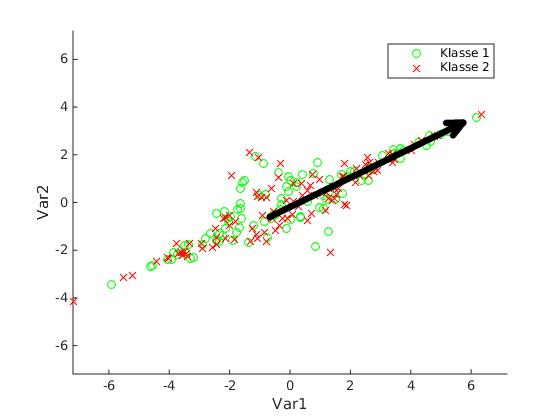
\includegraphics[width=0.5\textwidth]{data/img1_pc.jpg}
		
	\begin{enumerate}[1.]
		\item Bietet sich im Allgemeinen eine Dimensionsreduktion auf den PC-Vektor an?
		
		Die Daten befinden sich relativ gut auf einer Geraden, also bietet sich eine Dimensionsreduktion an.
		
		\item Ist dies für die Klassifikation förderlich?
		
		Nein ist es nicht, durch eine Reduktion sind die Klassen nicht gut unterscheidbar.
		
	\end{enumerate}
	
	\item \hfill
	
	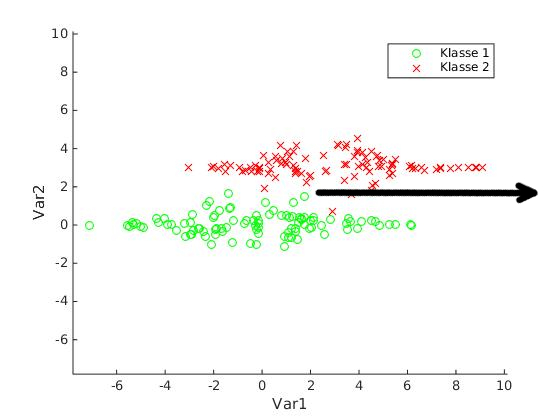
\includegraphics[width=0.5\textwidth]{data/img2_pc.jpg}
	
	\begin{enumerate}[1.]
		\item Bietet sich im Allgemeinen eine Dimensionsreduktion auf den PC-Vektor an?
		
		Die Daten befinden sich tendenziell eher auf einer Linie. Eine Dimensionsreduktion könnte sich durchaus anbieten, falls der Verlust des Var2 Wertes hinnehmbar ist, denn die Daten unterscheiden sich stark im Bezug auf den Var1 Wert.
		
		\item Ist dies für die Klassifikation förderlich?
		
		Nein ist es nicht, durch eine Reduktion sind die Klassen nicht gut unterscheidbar.
		
	\end{enumerate}
	
	\item \hfill
	
	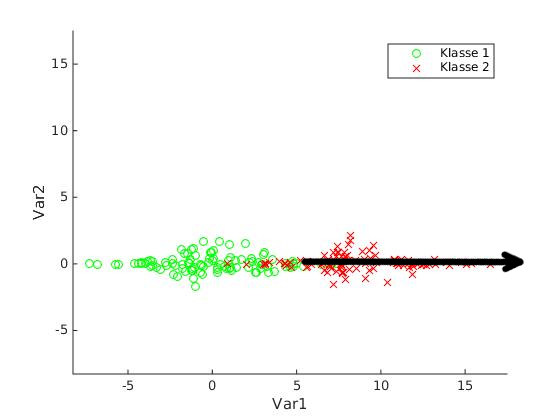
\includegraphics[width=0.5\textwidth]{data/img3_pc.jpg}
	
	\begin{enumerate}[1.]
		\item Bietet sich im Allgemeinen eine Dimensionsreduktion auf den PC-Vektor an?
		
		Ja, die Daten unterscheiden sich hauptsächlich im Wert von Var1, eine Dimensionsreduktion bietet sich also an.
		
		\item Ist dies für die Klassifikation förderlich?
		
		Ja ist es, durch eine Reduktion sind die Klassen immer noch gut unterscheidbar.
		
	\end{enumerate}
	
	\item \hfill
	
	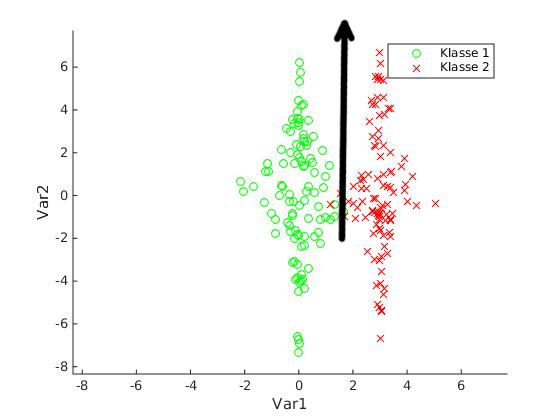
\includegraphics[width=0.5\textwidth]{data/img4_pc.jpg}
	
	\begin{enumerate}[1.]
		\item Bietet sich im Allgemeinen eine Dimensionsreduktion auf den PC-Vektor an?
		
		Die Daten befinden sich tendenziell eher auf einer Linie. Eine Dimensionsreduktion könnte sich durchaus anbieten, falls der Verlust des Var1 Wertes hinnehmbar ist, denn die Daten unterscheiden sich stark im Bezug auf den Var2 Wert.
		
		\item Ist dies für die Klassifikation förderlich?
		
		Nein ist es nicht, durch eine Reduktion sind die Klassen nicht gut unterscheidbar.
		
	\end{enumerate}
	
\end{enumerate}


\section{Principal Component Analysis – 2}

\textbf{Welche PCs enthalten zusammen mindestens  95\% der Streuung?}\\
Komponente 1 und 2 enthalten 97.6\% der Streuung (die erste Komponente allein macht  ca. 92\% aus).
Die erste und zweite Komponente werden auf jeden Fall benötigt um die 95\% zu erreichen. 
Komponente 3 und 4 haben fast keinen Einfluss auf die Streuung.\\


\textbf{Plotten des Ergebnisses}\\

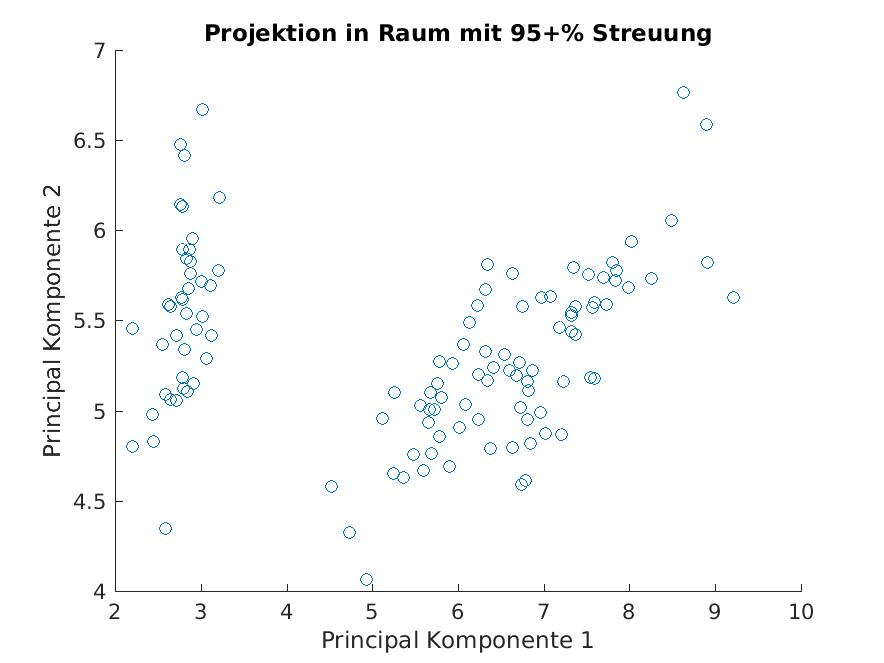
\includegraphics[width=0.75\textwidth]{plots/plotresultE.jpg}

\textbf{Ergibt die PCA in diesem Zusammenhang Sinn? Warum oder warum nicht?}\\
Ja - wir sehen, dass es möglich ist unseren Datensatz durch eine Projektion in die entsprechende Richtungen (erste beiden Principal Components) zu separieren, in diesen beiden Richtungen/Komponenten ist die meiste Information des Datensatzes enthalten.
Fuer eine Klassifikation bzw. Zuordnung der Pflanzen anhand der Merkmale macht diese Projektion aber keinen Sinn mehr. 
   
\section{Linear Discriminant Analysis}

\textbf{Plottet die originalen Datensätze und deren Projektionen und beurteilt bzw. begründet die Resultate.}

%\includegraphics[width=0.75\textwidth]{plots/PlotName.jpg}

\end{document}
